\documentclass[finnish,]{book}
\usepackage{lmodern}
\usepackage{amssymb,amsmath}
\usepackage{ifxetex,ifluatex}
\usepackage{fixltx2e} % provides \textsubscript
\ifnum 0\ifxetex 1\fi\ifluatex 1\fi=0 % if pdftex
  \usepackage[T1]{fontenc}
  \usepackage[utf8]{inputenc}
\else % if luatex or xelatex
  \ifxetex
    \usepackage{mathspec}
  \else
    \usepackage{fontspec}
  \fi
  \defaultfontfeatures{Ligatures=TeX,Scale=MatchLowercase}
\fi
% use upquote if available, for straight quotes in verbatim environments
\IfFileExists{upquote.sty}{\usepackage{upquote}}{}
% use microtype if available
\IfFileExists{microtype.sty}{%
\usepackage{microtype}
\UseMicrotypeSet[protrusion]{basicmath} % disable protrusion for tt fonts
}{}
\usepackage[margin=1in]{geometry}
\usepackage{hyperref}
\hypersetup{unicode=true,
            pdftitle={Bookdown-dokumetti - testi 1},
            pdfauthor={Jussi Hirvonen},
            pdfborder={0 0 0},
            breaklinks=true}
\urlstyle{same}  % don't use monospace font for urls
\ifnum 0\ifxetex 1\fi\ifluatex 1\fi=0 % if pdftex
  \usepackage[shorthands=off,main=finnish]{babel}
\else
  \usepackage{polyglossia}
  \setmainlanguage[]{finnish}
\fi
\usepackage{natbib}
\bibliographystyle{apalike}
\usepackage{color}
\usepackage{fancyvrb}
\newcommand{\VerbBar}{|}
\newcommand{\VERB}{\Verb[commandchars=\\\{\}]}
\DefineVerbatimEnvironment{Highlighting}{Verbatim}{commandchars=\\\{\}}
% Add ',fontsize=\small' for more characters per line
\usepackage{framed}
\definecolor{shadecolor}{RGB}{248,248,248}
\newenvironment{Shaded}{\begin{snugshade}}{\end{snugshade}}
\newcommand{\AlertTok}[1]{\textcolor[rgb]{0.94,0.16,0.16}{#1}}
\newcommand{\AnnotationTok}[1]{\textcolor[rgb]{0.56,0.35,0.01}{\textbf{\textit{#1}}}}
\newcommand{\AttributeTok}[1]{\textcolor[rgb]{0.77,0.63,0.00}{#1}}
\newcommand{\BaseNTok}[1]{\textcolor[rgb]{0.00,0.00,0.81}{#1}}
\newcommand{\BuiltInTok}[1]{#1}
\newcommand{\CharTok}[1]{\textcolor[rgb]{0.31,0.60,0.02}{#1}}
\newcommand{\CommentTok}[1]{\textcolor[rgb]{0.56,0.35,0.01}{\textit{#1}}}
\newcommand{\CommentVarTok}[1]{\textcolor[rgb]{0.56,0.35,0.01}{\textbf{\textit{#1}}}}
\newcommand{\ConstantTok}[1]{\textcolor[rgb]{0.00,0.00,0.00}{#1}}
\newcommand{\ControlFlowTok}[1]{\textcolor[rgb]{0.13,0.29,0.53}{\textbf{#1}}}
\newcommand{\DataTypeTok}[1]{\textcolor[rgb]{0.13,0.29,0.53}{#1}}
\newcommand{\DecValTok}[1]{\textcolor[rgb]{0.00,0.00,0.81}{#1}}
\newcommand{\DocumentationTok}[1]{\textcolor[rgb]{0.56,0.35,0.01}{\textbf{\textit{#1}}}}
\newcommand{\ErrorTok}[1]{\textcolor[rgb]{0.64,0.00,0.00}{\textbf{#1}}}
\newcommand{\ExtensionTok}[1]{#1}
\newcommand{\FloatTok}[1]{\textcolor[rgb]{0.00,0.00,0.81}{#1}}
\newcommand{\FunctionTok}[1]{\textcolor[rgb]{0.00,0.00,0.00}{#1}}
\newcommand{\ImportTok}[1]{#1}
\newcommand{\InformationTok}[1]{\textcolor[rgb]{0.56,0.35,0.01}{\textbf{\textit{#1}}}}
\newcommand{\KeywordTok}[1]{\textcolor[rgb]{0.13,0.29,0.53}{\textbf{#1}}}
\newcommand{\NormalTok}[1]{#1}
\newcommand{\OperatorTok}[1]{\textcolor[rgb]{0.81,0.36,0.00}{\textbf{#1}}}
\newcommand{\OtherTok}[1]{\textcolor[rgb]{0.56,0.35,0.01}{#1}}
\newcommand{\PreprocessorTok}[1]{\textcolor[rgb]{0.56,0.35,0.01}{\textit{#1}}}
\newcommand{\RegionMarkerTok}[1]{#1}
\newcommand{\SpecialCharTok}[1]{\textcolor[rgb]{0.00,0.00,0.00}{#1}}
\newcommand{\SpecialStringTok}[1]{\textcolor[rgb]{0.31,0.60,0.02}{#1}}
\newcommand{\StringTok}[1]{\textcolor[rgb]{0.31,0.60,0.02}{#1}}
\newcommand{\VariableTok}[1]{\textcolor[rgb]{0.00,0.00,0.00}{#1}}
\newcommand{\VerbatimStringTok}[1]{\textcolor[rgb]{0.31,0.60,0.02}{#1}}
\newcommand{\WarningTok}[1]{\textcolor[rgb]{0.56,0.35,0.01}{\textbf{\textit{#1}}}}
\usepackage{longtable,booktabs}
\usepackage{graphicx,grffile}
\makeatletter
\def\maxwidth{\ifdim\Gin@nat@width>\linewidth\linewidth\else\Gin@nat@width\fi}
\def\maxheight{\ifdim\Gin@nat@height>\textheight\textheight\else\Gin@nat@height\fi}
\makeatother
% Scale images if necessary, so that they will not overflow the page
% margins by default, and it is still possible to overwrite the defaults
% using explicit options in \includegraphics[width, height, ...]{}
\setkeys{Gin}{width=\maxwidth,height=\maxheight,keepaspectratio}
\IfFileExists{parskip.sty}{%
\usepackage{parskip}
}{% else
\setlength{\parindent}{0pt}
\setlength{\parskip}{6pt plus 2pt minus 1pt}
}
\setlength{\emergencystretch}{3em}  % prevent overfull lines
\providecommand{\tightlist}{%
  \setlength{\itemsep}{0pt}\setlength{\parskip}{0pt}}
\setcounter{secnumdepth}{5}
% Redefines (sub)paragraphs to behave more like sections
\ifx\paragraph\undefined\else
\let\oldparagraph\paragraph
\renewcommand{\paragraph}[1]{\oldparagraph{#1}\mbox{}}
\fi
\ifx\subparagraph\undefined\else
\let\oldsubparagraph\subparagraph
\renewcommand{\subparagraph}[1]{\oldsubparagraph{#1}\mbox{}}
\fi

%%% Use protect on footnotes to avoid problems with footnotes in titles
\let\rmarkdownfootnote\footnote%
\def\footnote{\protect\rmarkdownfootnote}

%%% Change title format to be more compact
\usepackage{titling}

% Create subtitle command for use in maketitle
\newcommand{\subtitle}[1]{
  \posttitle{
    \begin{center}\large#1\end{center}
    }
}

\setlength{\droptitle}{-2em}

  \title{Bookdown-dokumetti - testi 1}
    \pretitle{\vspace{\droptitle}\centering\huge}
  \posttitle{\par}
    \author{Jussi Hirvonen}
    \preauthor{\centering\large\emph}
  \postauthor{\par}
      \predate{\centering\large\emph}
  \postdate{\par}
    \date{2018-07-23 (Versio 3.01)}


\usepackage{amsthm}
\newtheorem{theorem}{Theorem}[chapter]
\newtheorem{lemma}{Lemma}[chapter]
\theoremstyle{definition}
\newtheorem{definition}{Definition}[chapter]
\newtheorem{corollary}{Corollary}[chapter]
\newtheorem{proposition}{Proposition}[chapter]
\theoremstyle{definition}
\newtheorem{example}{Example}[chapter]
\theoremstyle{definition}
\newtheorem{exercise}{Exercise}[chapter]
\theoremstyle{remark}
\newtheorem*{remark}{Remark}
\newtheorem*{solution}{Solution}
\begin{document}
\maketitle

{
\setcounter{tocdepth}{1}
\tableofcontents
}
\hypertarget{bookdown-paketin-testidokumentti}{%
\chapter{Bookdown-paketin
testidokumentti}\label{bookdown-paketin-testidokumentti}}

Esimerkki Rmarkdownin ja bookdown-paketin käytöstä. Kuvat, taulukot ja
kaavat numeroidaan ja niihin voi viitata tekstissä. Lähdeviitteet
toimivat, myös ne joissa on ns.

A sample document using RMarkdown with bookdown-package to do
statistical analysis and publish a report in html and pdf formats.

\hypertarget{johdanto}{%
\chapter{Johdanto}\label{johdanto}}

\hypertarget{alkutoimia}{%
\section{Alkutoimia}\label{alkutoimia}}

Ero YAML-headerissa lang-parametri (lang: fi). (verrattuna
bookdown-demoon). Bookdown-demossa lisäksi output: pdf\_document, mutta
lienee tarpeeton kun kaksi outputformaattia annettu
output.yaml-tiedostossa

20.7.2018 poistetaan tästä dokkarista child-item - jutut. Jätetään
r-pakettien lataus.

Bookdown - formaatissa ``juuritiedoston'' indexBD.Rmd tekstit eivät
tulostu jos siellä ei ole luvun (chapter) aloittavaa ensimmäisen tason
otsikkoa.Siellä on YAML-headeri (metadata).

Lisää YAML-parametreja voi antaa tiedostoissa \_bookdown.yml ja
\_output.yml. Nämä lienee välittyvät Pandocille?

Bookdown - demon esimerkkitiedostot ovat nämä:

ouput.yml (huomaa, että \_ - merkki jätetty pois!) (tässä oli
bookdown-demo-paketin yml-tiedostot, poistin 3.7.2018)

\hypertarget{tarkeimmat-ohjelmistot}{%
\section{Tärkeimmät ohjelmistot}\label{tarkeimmat-ohjelmistot}}

\begin{Shaded}
\begin{Highlighting}[]
\KeywordTok{system}\NormalTok{(}\StringTok{"pdflatex --version"}\NormalTok{)}
\CommentTok{#getwd()}

\NormalTok{rmarkdown}\OperatorTok{::}\KeywordTok{pandoc_version}\NormalTok{()}
\end{Highlighting}
\end{Shaded}

\begin{verbatim}
## [1] '2.2.1'
\end{verbatim}

Viimeinen rivi kertoo pandoc-version.

\hypertarget{muutoksia-ja-tilannetietoja}{%
\section{Muutoksia ja
tilannetietoja}\label{muutoksia-ja-tilannetietoja}}

Nyt toimii gitbook ja pdf\_book tulostusformaatteina. Molemmat ovat
html-paketteja, ja tarvitsevat ehkä r-datahakemistosta (omalta koneelta)
libs-hakemiston jQuery- ja Gitbook-paketit (javaskriptiä ja
css-tyylitiedostoja).

Bookdown-tulostuksessa voisi käyttää ``one document'' - optioita
(funktioita).

3.7.2018 PDF-tulostuksen säätöä, nyt saadaan jo virheilmoituksiakin!
Piti tallentaa utf-8 - muodossa kertaalleen. Tulostus kaatuu valituksiin
puuttuvista \$-merkeistä kaavoissa (test\_kaavat1.rmd). TeX-tiedoston
voi kääntää PDF:ksi, mutta kaavat sekaisin ja paljon muutakin. Esim.
sisällysluettelo.

Merkistöt olivat pielessä (ei utf-8!), ja samoin test1\_preamble.tex
-tiedosto. Laitoin kuntoon, nyt asiallinen virheilmoitus:

! LaTeX Error: Two documentclass or documentstyle commands.

Error: Failed to compile indexBD.tex. See indexBD.log for more info.
Execution halted Poistetaan test1\_preambe.tex eka rivi kokonaan: \%
documentclass{[}12pt,a4paper,leqno{]} (alusta puuttuu takakeno) \%
dispositiopaperista, poistettiin ekalta riviltä \{article\} Lisäksi
usepackage{[}\textbf{utf8}{]}\{inputenc\}.

LaTeX Font Info: Redeclaring font encoding T1 on input line 48. ))

! LaTeX Error: Option clash for package babel.

Palautetaan eka rivi, documeteclass \{book\}. Taas virheilmoitus ! LaTeX
Error: Two documentclass or documentstyle commands. Poistetaan eka rivi.
Ja sama virheilmoitus ``option clash''.

Pahin virhe: equation-tägien välissä ei saa olla tyhjiä rivejä! Ongelmia
on myös lähdeluettelon aakkostuksessa, Å-ä- ö näyttävät aakkostuvan
kuten A, a ja o. Pitää testailla vielä.

\hypertarget{kaavat-ja-matemattiset-merkinnat}{%
\chapter{Kaavat ja matemattiset
merkinnät}\label{kaavat-ja-matemattiset-merkinnat}}

Kaavat on esitettävä bookdown-paketin määrityksillä. Viittausnimien on
oltava yksikäsitteisiä koko dokumentissa, jos käytetään ``merge and
knit'' menetelmää. Jos taas jokainen lapsidokumentti on ``itsenäinen''
(``knit and merge''), tämä koskee vain kyseistä dokumenttia (kts.
Bookdown - webkirja).

\hypertarget{kahden-luokittelumuuttuja-taulukko}{%
\section{Kahden luokittelumuuttuja
taulukko}\label{kahden-luokittelumuuttuja-taulukko}}

Kahden luokittelumuuttujan riippuvuutta voidaan testata \(\chi^{2}\) -
testillä. Testisuure saadaan laskemalla yhteen jokaisen solun
havaittujen ja odotetettujen (riippumattomuushypoteesi) frekvenssien
erotukset muodossa

\begin{equation}
  \chi^{2} = \frac{(havaittu - odotettu)^2} {odotettu}
  \label{eq:khii21}
\end{equation}

Tämä voidaan esittää ca:han sopivammalla tavalla parilla muunnoksella,
jolloin saamme riveittäin vastaavat termit rivisummalla painotettuna:

\begin{equation}
  rivisumma \times \frac{(havaittu \: riviprofiili - odotettu \: riviprofiili)^2} {odotettu \: riviprofiili}
  \label{eq:khii22}
\end{equation}

Kun jaamme nämä tekijät havaintojen kokonaismäärällä \(n\), rivisumma
muuntuu rivin massaksi, ja niiden summa muotoon \(\frac{\chi^{2}}{n}\).

\begin{equation}
 \frac{\chi^{2}}{n} = \phi^{2}
 \label{eq:inert1}
\end{equation}

Tunnusluku \(\phi^{2}\) on korrespondenssianalyysissä kokonaisinertia
(total inertia). Se kuvaa, kuinka paljon varianssia taulukossa on ja on
riippumaton havaintojen lukumäärästä. Tilastotieteessä tunnusluvulla on
useita vaihtoehtoisia nimiä (esim. mean square contingency coefficient),
ja sen neliöjuurta kutsutaan \(\phi\) - kertoimeksi.

Tässä siirrytään kahden luokittelumuuttujan taulukosta suhteellisten
frekvenssien taulukkoon, ja pieni pohdinta taulukoista yleensä olisi
paikallaan. Yhtälöihin voi viitata \eqref{eq:khii21} . Kokeillaan vielä,
toimivatko kirjallisuusviittet, kuten tärkeä lähde\citep{RefWorks:55}.

\hypertarget{taulukot-ja-kuvat}{%
\chapter{Taulukot ja kuvat}\label{taulukot-ja-kuvat}}

Tähän taulukoita ja kuvia, esimerkkiaineistoilla.

Kirjallisuutta on myös \citep{RefWorks:68}, ja \citep{RefWorks:57}
esittelee geometrisen tulkinnan peruskäsitteet yksinkertaisen kahden
luokittelumuuttujan korrespondenssianalyysin avaulla. Mitenköhän skandit
toimivat lähteissä, bib-tiedostossa on niitä myös escape-muodossa (katso
esim. \citep{RefWorks:100}, kritiikkiä on esittänyt
\citep{RefWorks:110})

Viitteet saa tulostusasetuksilla yhdelle sivulle, oletuksena on
viitteiden esittäminen jokaisen sivun alareunassa.

\hypertarget{taulukoita}{%
\section{Taulukoita}\label{taulukoita}}

Tästä poistettu koodilohko data\_1, ei tarvita jos ca-paketti on
ladattu. Ja alaviiva on aikanakin ref-labeleissa kielletty.
Koodilohkojen nimissä taitaa olla sallittu?

Taulukot tulostetaan funktiolla knitr::kable(). Taulukko numeroidaan ja
se saa automaattisesti labelin etutunnisteella `tab', ja siihen
liitetään chunk-label (esim alla tab:smoketable1).

Tämä koodipätkä ei antaa yhden kappaleen esikatselussa virheilmoituksen,
``smoke''-dataa ei löydy.

\begin{Shaded}
\begin{Highlighting}[]
\NormalTok{knitr}\OperatorTok{::}\KeywordTok{kable}\NormalTok{(smoke[,}\DecValTok{1}\OperatorTok{:}\DecValTok{4}\NormalTok{], }\DataTypeTok{booktabs =} \OtherTok{TRUE}\NormalTok{,}
  \DataTypeTok{caption =} \StringTok{'CA-paketin smoke-data (keinotekoinen)'}
\NormalTok{)}
\end{Highlighting}
\end{Shaded}

\begin{table}

\caption{\label{tab:smoketable1}CA-paketin smoke-data (keinotekoinen)}
\centering
\begin{tabular}[t]{lrrrr}
\toprule
  & none & light & medium & heavy\\
\midrule
SM & 4 & 2 & 3 & 2\\
JM & 4 & 3 & 7 & 4\\
SE & 25 & 10 & 12 & 4\\
JE & 18 & 24 & 33 & 13\\
SC & 10 & 6 & 7 & 2\\
\bottomrule
\end{tabular}
\end{table}

\begin{Shaded}
\begin{Highlighting}[]
\CommentTok{# Taulukkoon viittaaminen tekstissä \textbackslash{}@ref(label)}
\end{Highlighting}
\end{Shaded}

Taulukossa \ref{tab:smoketable1} on kahden luokittelumuuttujan
keinotekoinen esimerkkiaineisto tupakonnin määrästä henkilöstöryhmittäin
(SM = senior managemet, JM = junior management, SE ja JE vastaavasti
ryhmälle employee, SC = secretary).

Useampi taulukko saadaan taulukkoympäristöön (table environment)
yhdistämällä data-objektit listaksi.

\begin{Shaded}
\begin{Highlighting}[]
\CommentTok{# riviprofiilit}
\NormalTok{smoke.rpro <-}\StringTok{ }\NormalTok{smoke }\OperatorTok{/}\StringTok{ }\KeywordTok{rowSums}\NormalTok{ (smoke)}
\CommentTok{# keskiarvoprofiili}
\NormalTok{smoke.avrpro <-}\StringTok{ }\KeywordTok{colSums}\NormalTok{(smoke) }\OperatorTok{/}\StringTok{ }\KeywordTok{sum}\NormalTok{(smoke)}

\NormalTok{knitr}\OperatorTok{::}\KeywordTok{kable}\NormalTok{(}
  \KeywordTok{list}\NormalTok{(smoke.rpro, }\KeywordTok{t}\NormalTok{(smoke.avrpro)   ), }\DataTypeTok{digits =} \DecValTok{3}\NormalTok{,}
  \DataTypeTok{caption =} \StringTok{'Riviprofiilit ja keskiarvoprofiili'}\NormalTok{, }\DataTypeTok{booktabs =} \OtherTok{TRUE}
\NormalTok{)}
\end{Highlighting}
\end{Shaded}

\begin{table}
\caption{\label{tab:smoketable2}Riviprofiilit ja keskiarvoprofiili}

\centering
\begin{tabular}[t]{lrrrr}
\toprule
  & none & light & medium & heavy\\
\midrule
SM & 0.364 & 0.182 & 0.273 & 0.182\\
JM & 0.222 & 0.167 & 0.389 & 0.222\\
SE & 0.490 & 0.196 & 0.235 & 0.078\\
JE & 0.205 & 0.273 & 0.375 & 0.148\\
SC & 0.400 & 0.240 & 0.280 & 0.080\\
\bottomrule
\end{tabular}
\centering
\begin{tabular}[t]{rrrr}
\toprule
none & light & medium & heavy\\
\midrule
0.316 & 0.233 & 0.321 & 0.13\\
\bottomrule
\end{tabular}
\end{table}

Taulukossa \ref{tab:smoketable2} on laskettu jokaisen rivin
riviprofiilit. Ne saadan kun rivin luvut jaetaan rivin summalla. Yhden
rivin taulukossa on esitetty riviprofiilien keskikarvo, sarakesummat
jaettuna koko taulukon havaintojen lukumäärällä. Sen prosenttiluvut
kertovat tupakoititapojen jakauman koko henkilöstössä.

Jos PDF-tulostuksessa ei haluta ns. kelluvaa taulukkoa (float), voi
kable-funktiossa käyttää LaTeXin pakettia longtable. Silloin on myös
muistettava ottaa paketti käyttöön (usepackage\{\}) LaTeX -
pohjatiedostossa (preamble).

Pandoc tukee monia Markdownin taulukkotyyppejä. Viittaaminen vaaati
labeloidun otsikon, ja sen on oltava otsikkotestin alussa
määrämuotoisena (esim. ab:hienotaulu). Tämä vaatii tarkkuutta, jos
taulukon pitää toimia html- ja LaTex-outputissa. kable-funktiota
kannattaa käyttää!

\hypertarget{korrespondenssianalyysin-numeeriset-tulokset-taulukoina}{%
\section{Korrespondenssianalyysin numeeriset tulokset
taulukoina}\label{korrespondenssianalyysin-numeeriset-tulokset-taulukoina}}

Korrespondenssianalyysin idea on vähentää aineiston dimensioita, ja
esittää taulukon rivien ja sarakkeiden riippuvuudet yleensä
kaksiulotteisena karttana.

\begin{Shaded}
\begin{Highlighting}[]
\NormalTok{smokeCA <-}\StringTok{ }\KeywordTok{ca}\NormalTok{(smoke)}
\NormalTok{temp1 <-}\StringTok{ }\NormalTok{smokeCA }
\NormalTok{numres1CA1 <-}\StringTok{ }\KeywordTok{summary}\NormalTok{(smokeCA)}
\CommentTok{#str(smokeCA)}
\CommentTok{#knitr::kable( smokeCA,}
\CommentTok{#  digits = 3,}
\CommentTok{#  caption = 'Riviprofiilit ja keskiarvoprofiili', booktabs = TRUE}
\CommentTok{#)}
\CommentTok{#str(temp1)}
\CommentTok{#stargazer(temp2$rows, type = "text", title = "CA-tuloksia")}
\CommentTok{# LateX-tulostuksessa float vaatii jotain tällaista:Table: (\textbackslash{}#tab:cataul1) }
\CommentTok{#str(temp2)}
\CommentTok{#str(temp2$scree)}
\CommentTok{#temp2$scree}
\end{Highlighting}
\end{Shaded}

Taulukot ovatkin aika vaikeita, tulostiedoista! Stargazer toki tekee
monenlaista, mutta kun kyse on hyvin yksinkertaisista tulostaulukoista
kablen pitäisi toimia.

Kokeillaan summary(smokeCA) - listan dataframe-olioden tulostusta
kablella. Voisi harkita funktiota, joka poimii CA:n tuloslistasta
sopivat objektit kable-funktiolle? Stargazer taas vaatisi (luultavasti)
jonkun ehdollisen tulostuksen (PDF ja html)?

\begin{Shaded}
\begin{Highlighting}[]
\NormalTok{knitr}\OperatorTok{::}\KeywordTok{kable}\NormalTok{( numres1CA1}\OperatorTok{$}\NormalTok{rows,}
    \DataTypeTok{digits =} \DecValTok{3}\NormalTok{,          }
    \DataTypeTok{caption =} \StringTok{'Korrespondenssianalyysin diagnostiikkaa - rivit'}\NormalTok{, }\DataTypeTok{booktabs =} \OtherTok{TRUE}
\NormalTok{)}
\end{Highlighting}
\end{Shaded}

\begin{table}

\caption{\label{tab:simpleCAtab1}Korrespondenssianalyysin diagnostiikkaa - rivit}
\centering
\begin{tabular}[t]{lrrrrrrrrr}
\toprule
name & mass &  qlt &  inr &  k=1 & cor & ctr &  k=2 & cor & ctr\\
\midrule
SM & 57 & 893 & 31 & -66 & 92 & 3 & -194 & 800 & 214\\
JM & 93 & 991 & 139 & 259 & 526 & 84 & -243 & 465 & 551\\
SE & 264 & 1000 & 450 & -381 & 999 & 512 & -11 & 1 & 3\\
JE & 456 & 1000 & 308 & 233 & 942 & 331 & 58 & 58 & 152\\
SC & 130 & 999 & 71 & -201 & 865 & 70 & 79 & 133 & 81\\
\bottomrule
\end{tabular}
\end{table}

Rivien ja sarakkeiden diagnotiikkataulukot eivät mahdu rinnakkain, siksi
ne tulostetaan erikseen.

\begin{Shaded}
\begin{Highlighting}[]
\NormalTok{knitr}\OperatorTok{::}\KeywordTok{kable}\NormalTok{( numres1CA1}\OperatorTok{$}\NormalTok{columns,}
    \DataTypeTok{digits =} \DecValTok{3}\NormalTok{,          }
    \DataTypeTok{caption =} \StringTok{'Korrespondenssianalyysin diagnostiikkaa - sarakkeet'}\NormalTok{, }\DataTypeTok{booktabs =} \OtherTok{TRUE}
\NormalTok{)}
\end{Highlighting}
\end{Shaded}

\begin{table}

\caption{\label{tab:simpleCAtab2}Korrespondenssianalyysin diagnostiikkaa - sarakkeet}
\centering
\begin{tabular}[t]{lrrrrrrrrr}
\toprule
name & mass &  qlt &  inr &  k=1 & cor & ctr &  k=2 & cor & ctr\\
\midrule
none & 316 & 1000 & 577 & -393 & 994 & 654 & -30 & 6 & 29\\
lght & 233 & 984 & 83 & 99 & 327 & 31 & 141 & 657 & 463\\
medm & 321 & 983 & 148 & 196 & 982 & 166 & 7 & 1 & 2\\
hevy & 130 & 995 & 192 & 294 & 684 & 150 & -198 & 310 & 506\\
\bottomrule
\end{tabular}
\end{table}

Taulukoiden \ref{tab:simpleCAtab1} ja \ref{tab:simpleCAtab2} luvut on
kerrottu tuhannella (``per milles'').

Dimensioiden ominaisarvot (eli niiden osuus kokonaisinertiasta) saadaan
ca-funktion tuloslistasta taulukoksi. Se esitetään joskus myös ns. scree
- kuvana, jos dimensoita on paljon ja joudutaan pohtimaan kuinka monta
valitaan (vaikea kysymys!).

\begin{Shaded}
\begin{Highlighting}[]
\NormalTok{knitr}\OperatorTok{::}\KeywordTok{kable}\NormalTok{( numres1CA1}\OperatorTok{$}\NormalTok{scree,}
    \DataTypeTok{digits =} \DecValTok{3}\NormalTok{,          }
    \DataTypeTok{caption =} \StringTok{'Korrespondenssianalyysin diagnostiikkaa - ominaisarvot'}\NormalTok{, }\DataTypeTok{booktabs =} \OtherTok{TRUE}
\NormalTok{)}
\end{Highlighting}
\end{Shaded}

\begin{table}

\caption{\label{tab:simpleCAscree}Korrespondenssianalyysin diagnostiikkaa - ominaisarvot}
\centering
\begin{tabular}[t]{rrrr}
\toprule
 & values & values2 & values3\\
\midrule
1 & 0.075 & 87.756 & 87.756\\
2 & 0.010 & 11.759 & 99.515\\
3 & 0.000 & 0.485 & 100.000\\
\bottomrule
\end{tabular}
\end{table}

Taulukko \ref{tab:simpleCAscree} vaatii selityksen, mutta kuvaa ei tässä
tapauksessa tarvita.

\hypertarget{kuvat}{%
\section{Kuvat}\label{kuvat}}

\textbf{chunk-optiot}

fig.cap: R plot - kuvat figure-ympäristöön, automaattiset labelit (fig:
+ koodipätkän label) ja niihin voi viitata.

fig.asp oikeaan arvoon 1.

\begin{Shaded}
\begin{Highlighting}[]
\KeywordTok{plot}\NormalTok{(smokeCA)}
\end{Highlighting}
\end{Shaded}

\begin{figure}
\centering
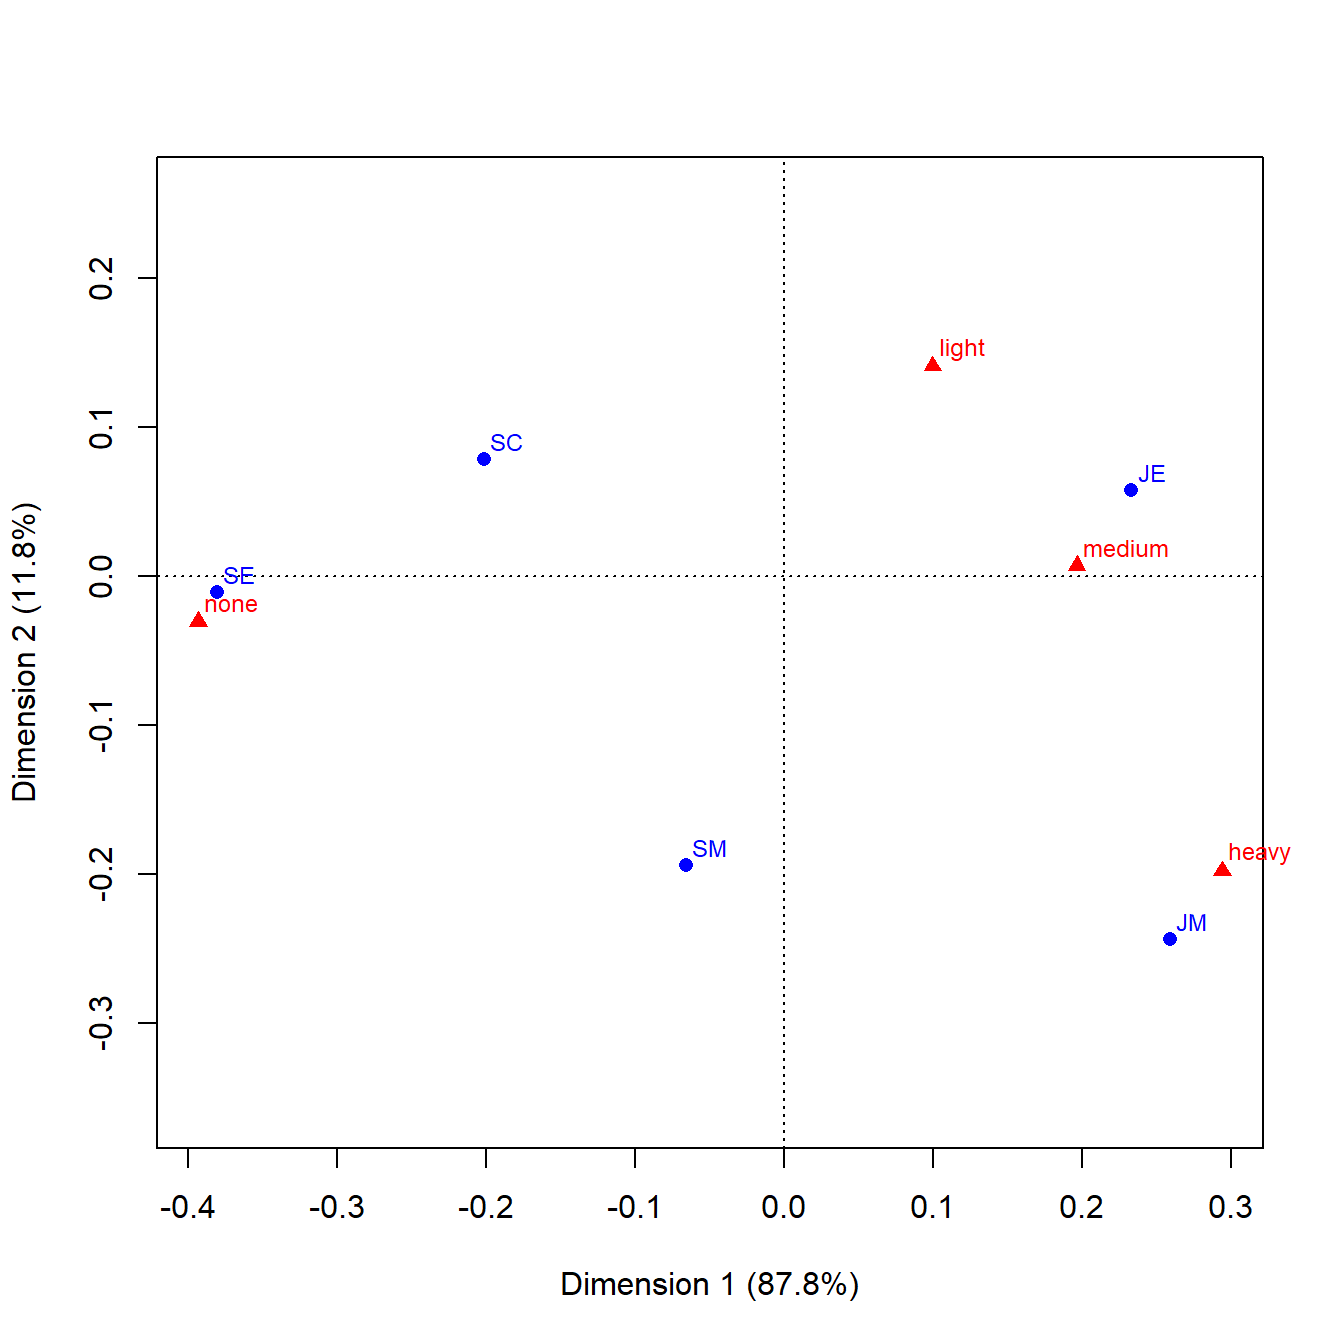
\includegraphics{bookdown-testi1_files/figure-latex/CAmap1-1.pdf}
\caption{\label{fig:CAmap1}CA-kartta}
\end{figure}

Kuviin (kuten \ref{fig:CAmap1}) ja taulukoihin voi viitata tekstissä.
Kuvan otsikko tulostuu kuvan alapuolelle, ehkä vähän huono idea?

Näköjään stargazer-kokeilu tulostusoptiolla ``html'' loi
R-projektihakemistoon kansion ja sinne png-kuvan. finnish.ldf tiedoston
muokkaus MikTeX:ssä tehty, mutta se ei vaikuta html-viiteotsikkoon.
Korjattu ``ehdollisessa viitesivussa'' viitteet.Rmd jossa
html-viiteluettelon otsikko annetaan.

Saisiko numeeristen tulosten scree-kuvan samalla tavalla kuvaksi?

\hypertarget{bookdown-ja-rmarkdown}{%
\chapter{Bookdown ja Rmarkdown}\label{bookdown-ja-rmarkdown}}

Bookdown- R-paketti ``paketoi'' RMarkdownin tulostutoiminnot (output) ja
sen monet säädettävät optiot. Samat Rmd-dokumentit saadaan koottua
moneen eri formaattiin: html- sivuiksi, PDF-dokumentiksi tai
Ebook-kirjaksi. Kaikissa tulostusvaihtoehdoissa on monia eri
vaihtoehtoja. Html-tulostuksessa voi valita yhden tai useamman
html-sivun lisäksi gitbook- tai Tufte- vaihtoehdon. Ne on toteutettu
css-tyylitiedostoilla ja JavaScript-kirjastoilla. Tässä on käytetty
gitbook-formaattia.

LaTeX-formaatti renderöidään jollain LaTeX-vaihtoehdolla
PDF-tiedostoksi. \textbf{ToDo} PDF-formaattejakin on useita variantteja,
mikä niistä. Tässä vaihtoehdossa konfigurointimahdollisuudet ovat
käytännössä rajattomat, sillä välitulosteena syntyvää TeX-tiedostoa voi
muokata ja muuntaa sen sitten PDF-muotoon.

Prosessissa on monta vaihtetta, ja eri parametrien yhteisvaikutusta on
vaikea hahmottaa.

\begin{Shaded}
\begin{Highlighting}[]
\NormalTok{knitr}\OperatorTok{::}\KeywordTok{include_graphics}\NormalTok{(}\StringTok{'BookdownProc.png'}\NormalTok{)}
\end{Highlighting}
\end{Shaded}

\begin{figure}

{\centering 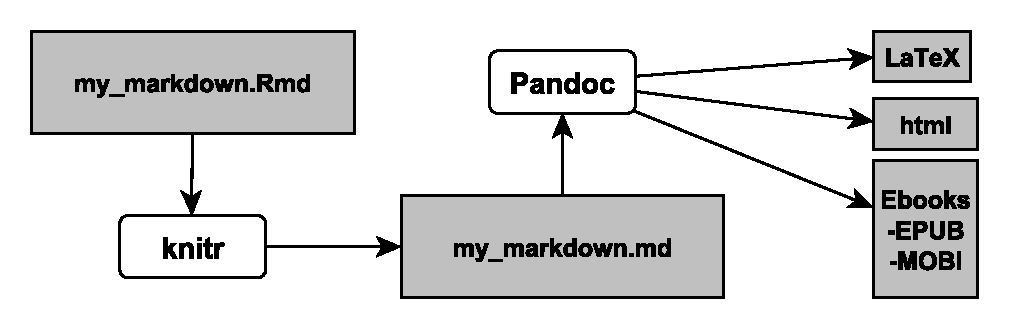
\includegraphics[width=0.5\linewidth]{BookdownProc} 

}

\caption{Tulostiedoston prosessointi}\label{fig:bdprocess}
\end{figure}

Perusopas bookdown paketin käyttöön on Yihui Xien
\href{https://bookdown.org/yihui/bookdown/}{``bookdown: Authoring Books
and Technical Documents with R Markdown''"}. Siinä pääidea on tuottaa
yhdellä Rmd-koodilla kuvan \ref{fig:bdprocess} kolme vaihtoehtoista
tulostiedostoa mahdollisimman yksinkertaisesti. Knitr- ohjelma ``kutoo''
Rmd-tiedoston r-koodilohkojen tulokset ja tekstin markdown-tiedostoksi
(md). Rmd-tiedostojen YAML-asetukset siirtyvät Pandocille, joka
täydentää niillä omia mallitiedostojaan (template).

Laajempi ja tarkempi opas ilmestyi 15.7.2018, kolmen kirjoittajan
\href{https://bookdown.org/yihui/rmarkdown/}{``R Markdown: The
Definitive Guide''}. Siinä eri asetusten hierarkia on kuvattu tarkemmin
ja selkeämmin. Tulostusvaihtoehtoja esitellään laajemmin, bookdown on
vain yksi luku.

R Studiolla alkuun pääse helposti, kun lataa bookdown-paketin, ja luo
uuden bookdown-projektin. Xien ensimmäisen kirjan alku-luvut ja uudemman
teoksen johdattelut auttavat jatkoon.

\bibliography{bdtest1.bib}


\end{document}
